\chapter{BACKGROUND AND RELATED WORK}
\label{chap:Literature}
    
Mobile robots are characterised by the ability to move in space, so the idea of placing a manipulator on mobile robotic platforms helps increase the workspace of the robotic manipulator and consequently reducing operating costs. Thus, a robotic manipulator mounted on a mobile platform is called a mobile (robotic) manipulator. The control of the mobile manipulators can be achieved in two ways \cite{Nassal1994}: the control of the manipulator and mobile base separately or the control of the mobile manipulator as a whole.

In addition, the control of the mobile manipulator is done separately, and thus, the following literature reviews for autonomous mobile robot navigation and robotic manipulator force estimation will be given separately in the following sections. Since the research on both topics is based on neural networks, a brief overview of its methods is given.

\section{Neural networks and deep learning}

\emph{Neural networks} (or sometimes termed, artificial neural networks) are a model of machine learning inspired by biological neural networks. It is a set of interconnected nodes, called neurons, and their processing power lies in the adaptable weights between neurons, which can change and adapt and consequently enable the neural network to ``learn''. Thus, the learning of neural networks is based on adapting those weights based on the provided training data.

Neural networks are mainly used for classification or regression tasks. In a neural network for classification, an input is classified as either belonging or not belonging to a class, called binary classification or as belonging to one of the multiple classes, called multi-class classification. On the other side, neural networks for regression produce an output value (or values, in the case of multi-output regression) on a continuous scale.

Most neural networks are organised into groups of neurons called layers and, depending on how the layers are connected, make different network architectures. Usually, the layers are stacked in a chain-like structure, making the layer a function of the previous layer. The first layer of the network is called the input layer, the final layer is called the output layer, while all other layers are called hidden layers because the training data is not presented to them.

\emph{Deep learning} is a subset of machine learning that uses (deep) neural networks in the process of learning. It is termed as ``deep'' since, usually, neural networks are considered deep because of having multiple layers. A good overview of deep learning methods is given in \cite{Haykin1999,Schmidhuber2015,Goodfellow2016}.

The goal of a neural network is to approximate some nonlinear function $f^{*}(\vx)$ using the training data (which can be noisy \cite{Goodfellow2016}). The training data provides appropriate examples $\vx$ along with a label or target\footnote{The term \emph{target} is commonly used when the neural network is used to solve regression problems, while the term \emph{label} is used when the neural network solves classification problem.} $y\approx f^{*}(\vx)$. The goal of the network is then to output a value close to $y$ when provided with $\vx$ at the input. It is not specified in which way should the hidden layers behave, so it is the goal of the learning algorithm to use the hidden layers optimally to produce the best approximation of $f^{*}$. The scalar-valued function $f^*(\vx)$ can easily be extended to vector-valued function $\vf^*(\vx)$ in the case of multi-class classification or multi-output regression.

When a neural network is trained, the weights and biases of each layer are learned by optimising a loss function. Thus, an appropriate loss function must be chosen regarding the task the neural network needs to perform. This choice usually comes to using a well-known per-example loss function, whose values are summed over training examples \cite{Goodfellow2016}. The most widely used loss functions include mean squared error (MSE)
\[
    L(\vx,\vy,\mW) = ||\vy-f(\vx,\mW)||^2
\]
for regression and cross-entropy between training data and model
\[
    L(\vx,\vy,\mW) = -\log p_{model}(\vy|\vx)
\]
for classification neural networks. Then, a cost function is formed as
\[
    J(\vtheta) = \frac{1}{m}\sum_{i=1}^m L(\vx^{(i)}, \vy^{(i)}, \vtheta)
    \label{Eq:CostFunction}\\
\]
which is then optimised to obtain optimal weights of the network. The optimisation is achieved using the backpropagation algorithm \cite{Rumelhart1986}. Here, a cost function gradient is propagated backwards through the neural network and minimised using an optimisation algorithm (in theory, any nonlinear optimisation algorithm). The algorithm used initially for this purpose was Gradient descent, which is very old and is attributed to Cauchy (developed in the mid 19th century). Its application in the field of nonlinear optimisation was studied in the mid-20th-century \cite{Curry1944}. Other, better-performing algorithms were developed by building upon it, and some of the most widely used ones in state-of-the-art approaches include SGD, RMSProp, Adam \cite{Kingma2014}, and Adagrad \cite{Duchi2011}.

One more important thing in neural networks learning is regularisation. It is a set of techniques that make learning algorithms generalise better (i.e., avoids overfitting) and converge faster. Different regularisation techniques can be applied, the most commonly used ones being $L^2$ regularisation, $L^1$ regularisation. These regularisation techniques penalise cost function defined in \cref{Eq:CostFunction} as follows
\[
    \tilde{J}(\vtheta)=J(\vtheta)+\frac{\lambda}{2m}\sum\|\vtheta\|^2
\]
for $L^2$ regularisation and
\[
    \tilde{J}(\vtheta)=J(\vtheta)+\frac{\lambda}{2m}\sum\|\vtheta\|_1
\]
for $L^1$ regularisation. If regularisation is used, then the regularised cost function $\tilde{J}(\vtheta)$ is optimised in place of $J(\vtheta)$ cost function from \cref{Eq:CostFunction}. One more interesting regularisation technique is dropout \cite{Srivastava2014}. This dropout technique does not penalise network weights, but at each iteration during training, randomly selected neurons (besides ones in the output layer) are ignored, together with their inbound and outbound connections, making each iteration with a different set of neurons that are adapted. The dropout usually results in better generalisation since it prevents overfitting due to dependencies between neurons being removed.

A brief overview of the essential neural network architectures and the ones used in the research will be given in the following subsections. First, the multilayer perceptron will be introduced, together with all other vital aspects, like the choice of activation functions and training procedure. Following this, other architectures that emerge from the multilayer perceptron will follow. 

Finally, all of the networks trained for this research were trained using Tensorflow \cite{Abadi2015}, a well-known open-source deep learning framework. Additionally, Keras \cite{Chollet2015} was used on top of Tensorflow to facilitate the training of neural networks.

\subsection{Multilayer perceptron}
\label{sec:MLP}

Multilayer perceptron (or Deep feedforward network) is the most basic deep learning model. In addition, it is the basis for many other important neural network architectures. In this architecture, each neuron in a layer is connected to every neuron in the following layer. This kind of layer is referred to as a ``dense layer'' or ``fully-connected layer'' in the literature. It is used in almost all neural network architectures, given the ability to learn by adapting the weights. The multilayer perceptron architecture scheme is shown in Figure \ref{fig:MLPArch}.

The network consists of the input layer, any number of hidden layers, and the output layer. With the introduction of hidden layers, the activation function must be chosen as well. The activation function plays a vital role in this neural network since it computes the layers' values. The activation must be nonlinear. Otherwise, the neural network will not be able to approximate nonlinear functions.

\begin{figure}
    \centering
    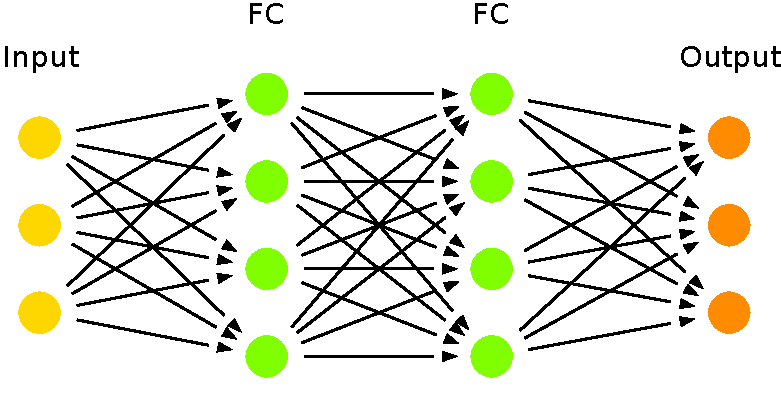
\includegraphics[width=0.9\textwidth]{slike/arch_mlp.pdf}
    \caption{The schematic of the multilayer perceptron architecture}
    \label{fig:MLPArch}
\end{figure}

The $i$-th hidden layer values depend on the values of the previous layer

\begin{equation}
    \vh_i = g_i\left(\mW_i^{\top}\vh_{i-1}+\vb_i \right)
\end{equation}
and the first hidden layer values depend on the network inputs (i.e., $\vh_0=\vx$). In the equation, $\mW_i$, $\vb_i$, $\vh_i$ are weight matrix, bias vector and layer value of the $i$-th layer, respectively, and $g_i(\cdot)$ is activation function, applied element-wise.

The activation function that is primarily used in state-of-the-art approaches to neural network training is Rectified linear unit (ReLU)

\[
    g(z)=\begin{cases}
    z & z>0\\
    0 & \textrm{otherwise}
    \end{cases}
\]
which has many benefits, including that it is computationally cheap. There are other activation functions, like logistic sigmoid
\[
    g(z)=\sigma(z)=\frac{1}{1+e^{-z}}
\]
and hyperbolic tangent
\[
    g(z)=\tanh(z)
\]

Both of these functions were used as activation functions before the introduction of ReLU. Therefore, these two functions are closely related and only differ in the codomain ($[0, 1]$ vs $[-1, 1]$), while they have the same shape. They are still used today in some applications and particular layers, like LSTM (introduced later).



\subsection{Convolutional neural networks}

Convolutional neural networks are a neural network architecture specialised for processing data that ``use convolution in place of general matrix multiplication in at least one of their layers'' \cite{Goodfellow2016}. They are often used to process grid-like data (1D grid for time series data or 2D pixels for image data). These networks are an extension of the multilayer perceptron, which assumes that neighbouring features are not independent, i.e., that they likely belong to the same temporal sequence (in the case of 1D convolution) or the same visual structure (in the case of 2D convolution). Convolutional neural networks are usually deeper than multilayer perceptrons because they are intended to use for the processing of more complex data.

The general architecture of convolutional neural networks is illustrated in Figure \ref{fig:ConvArch}. The image illustrates the general convolutional network and its types of layers without specifying whether it is a 1D or 2D convolution. Please note that neurons in the convolution layer are \emph{not} connected to each neuron in the following layer, but only to some of them. As it can also be seen, the convolutional layer(s) are followed by fully connected layers, as in the multilayer perceptron, and the functioning of this type of layer was introduced in Section \ref{sec:MLP}. Two-dimensional convolutional neural networks are left out of this review since they are primarily used for image processing which was not the part of this research in this dissertation.

\begin{figure}
    \centering
    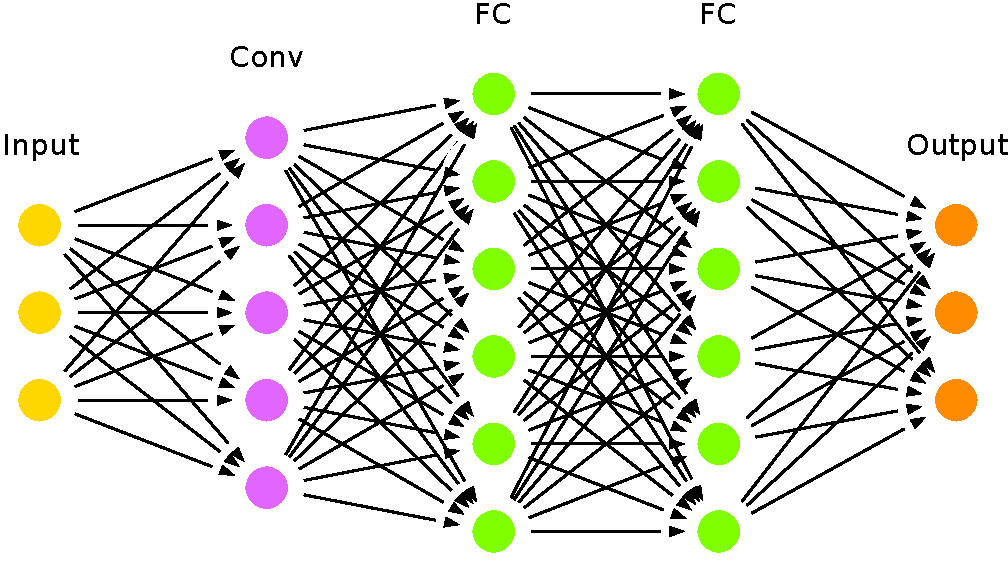
\includegraphics[width=0.8\textwidth]{slike/arch_conv.pdf}
    \caption{The schematic of typical convolutional neural network}
    \label{fig:ConvArch}
\end{figure}

The typical convolutional neural network begins with a convolution layer, usually followed by a pooling layer. After that, more convolution layers may follow, possibly followed by a pooling layer each. Fully connected layers then follow these layers as in the multilayer perceptron. This way of stacking layers enables convolutional networks to learn based on the features extracted by the convolution(s) rather than learning on raw inputs, which is the case of multilayer perceptrons.

The illustration of the one-dimensional convolution operation is shown in Figure \ref{fig:Conv1d}. First, the kernel ``slides'' along the input vector, and the output is a dot product between the ``covered'' part of the input and the kernel, producing a single scalar output. Then, the kernel moves one place right in the input, and the process is repeated until the kernel slides to the end of the input. The example in the figure shows a one-dimensional convolution with a single input sequence, but the example can be easily extended to multiple input sequences (i.e., channels). The same principle can be applied to 2D convolution with images as input, and if that is the case, the kernel will then be a matrix instead of a vector.

\begin{figure}
    \centering
    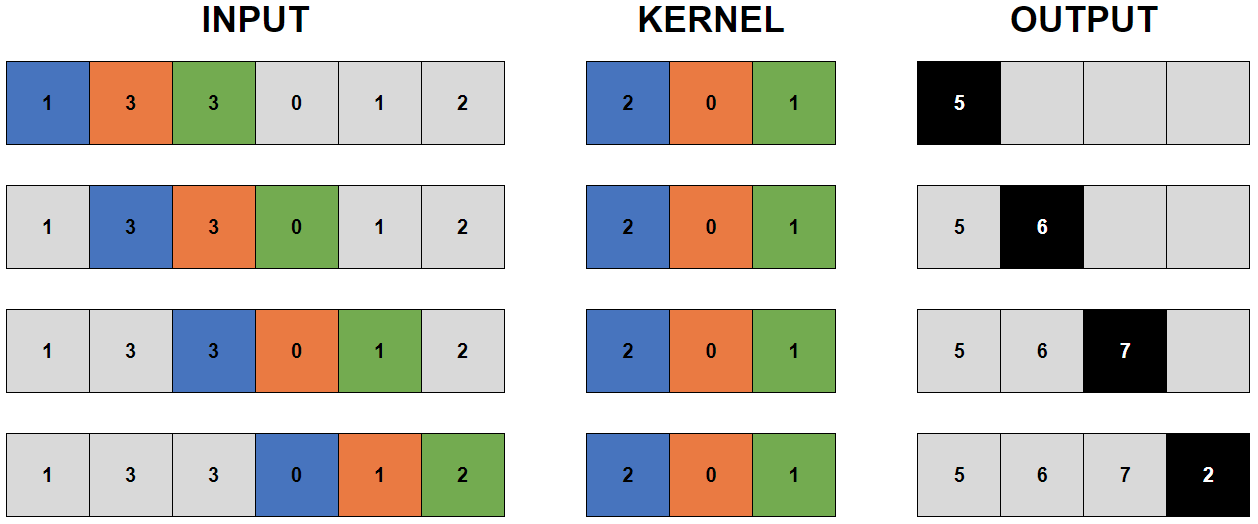
\includegraphics[width=0.9\textwidth]{slike/conv1d.png}
    \caption{The illustration of 1d convolution operation}
    \label{fig:Conv1d}
\end{figure}

One of the main characteristics of convolution layers is sparse weights, meaning that, unlike in multilayer perceptrons, not necessarily every unit is connected to all units in the next layer. This kind of connection is achieved because the kernel used in the convolution operation is smaller than the input, as is evident from the example in Figure \ref{fig:Conv1d}. Finally, the results of the convolution operation are activated using the activation function, most commonly ReLU.

Pooling layers may be used, but they are not mandatory in convolutional neural networks. They take the activated outputs of convolutional layers and produce output at a location that is a summary statistics about the location's surroundings (maximal or average values are the most used summary statistics in pooling layers). The pooling works by applying a sliding window of a specific size (smaller than that of the convolutional layer output). As a convolution operation might be viewed as one that extracts features from raw data, the pooling operation may keep the ``strongest'' or average feature among those extracted (using max pooling and average pooling, respectively). This way, downsampling of the signal is achieved.

\begin{figure}
    \centering
    \subfloat[Max pooling]{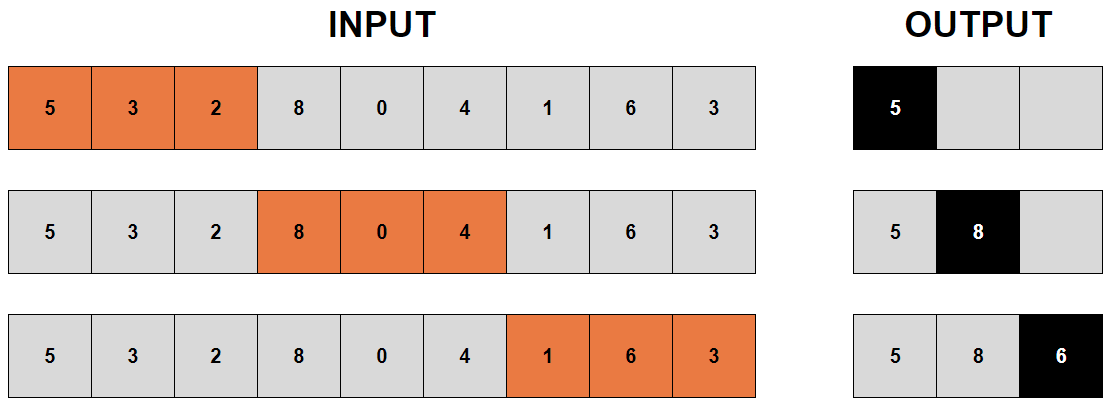
\includegraphics[height=4cm]{slike/pooling_max.png}}
    \vfill
    \subfloat[Average pooling]{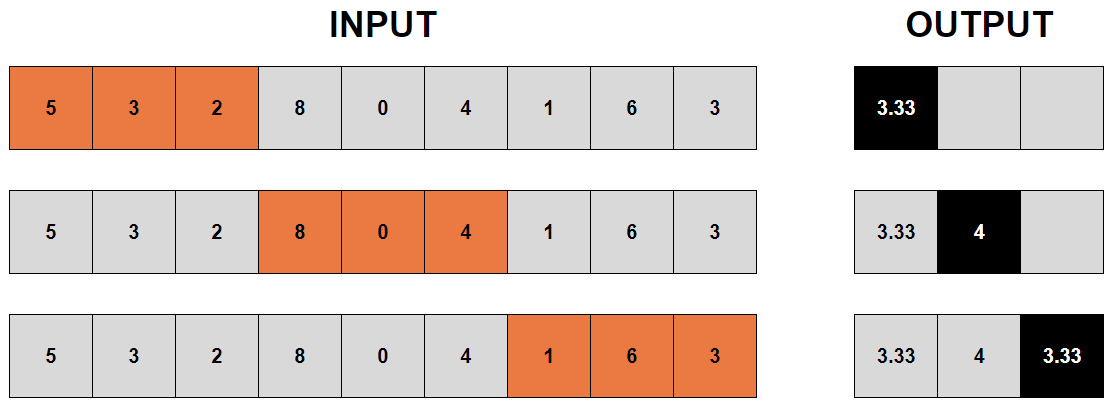
\includegraphics[height=4cm]{slike/pooling_avg.png}}
    \caption{The illustration of different types of pooling operation}
    \label{fig:Pooling}
\end{figure}

\subsection{Recurrent neural networks}

Recurrent neural networks (RNN) are used to process sequential data, most often temporal sequences. Most notable applications include signal processing and natural language processing. A recurrent neural network contains one or more recurrent layers at the beginning of the network, with fully connected layers following. It is similar to 1D convolutional neural networks in that both have a similar structure, but significant differences exist in how the data are processed in convolutional and recurrent layers.

The recurrent layer consists of \emph{cells} that feature a loop (or feedback), which makes a piece of information possible to persist between the training steps. This way, a recurrent neural network may be seen as multiple copies of the same network chained one after another. However, these networks are unable to handle ``long term dependencies'' \cite{Bengio1994}. Therefore, long Short Term Memory (LSTM) networks are introduced \cite{Hochreiter1997} to resolve this problem. This architecture came as a replacement to traditional recurrent neural networks and are nowadays used for most applications.

\begin{figure}
    \centering
    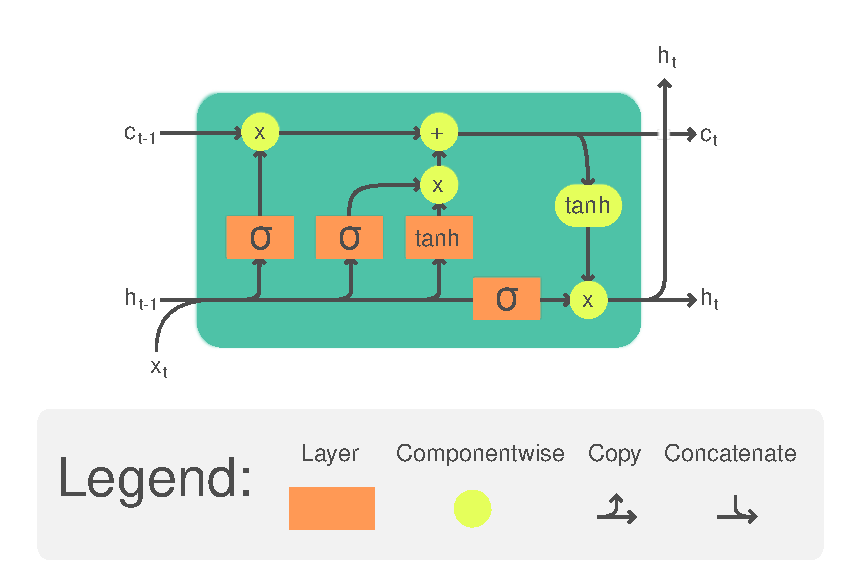
\includegraphics[width=\textwidth]{slike/LSTM_Cell.pdf}
    \caption[LSTM Cell]{\href{https://commons.wikimedia.org/wiki/File:LSTM_Cell.svg}{LSTM Cell} \copyright\,Guillaume Chevalier CC-BY-SA 4.0}
    \label{fig:LSTMCell}
\end{figure}

The LSTM cell is somewhat different from the classical RNN cell because its default behaviour is to learn long-term dependencies. A schematic of the LSTM cell is shown in Figure \ref{fig:LSTMCell}, where it can be seen that it contains four layers, of which three are activated with sigmoid activation and one with hyperbolic tangent activation (instead of one in classical RNN), that interact with the data. Furthermore, it has a state, which can be controlled using gates (horizontal line on top of the schematic in Figure \ref{fig:LSTMCell}, with input $c_{t-1}$ and output $c_t$). This way, the cell can decide whether a piece of information will be kept or discarded. More detailed insights into how LSTM cells work, along with the mathematical details, can be found in \cite{Olah2015}.

    
\section{Autonomous Mobile Robot Navigation}

Autonomous mobile robots are increasingly being used in dynamic (changing) environments \cite{Kunze2018,Guiochet2017,Ramachandram2017,BoninFont2008,Jarvis2008}. Due to the uncertain nature of such environments, robot behaviour should be adaptive to operate adequately with minimal or no human-operator effort. These environments range from air-, water- and ground-based ones to space-based ones \cite{Kunze2018,BoninFont2008}. This dissertation focuses on ground-based autonomous mobile robots, but some of its contributions and conclusions could easily be extended to other domains (like air and water). Thus, the term \emph{autonomous mobile robots} will refer to ground-based mobile platforms for this dissertation.

In order to move in space, mobile robots need to be equipped with appropriate navigation methods. Traditionally, navigation is usually a combination of three fundamental operations: localisation, path planning and mapping (and map comprehension). Localisation aims to estimate the current robot state based on sensor readings, which is a probabilistic procedure due to the dynamic environment. Thus, localisation provides a probability distribution that the robot is in a certain state. State-of-the-art localisation methods are based either on Extended Kalman Filter \cite{Jetto1999,Moore2015} (and its variants) or Monte Carlo Localisation \cite{Dellaert1999,Thrun2006}. The mapping is usually done using a procedure called Simultaneous Localisation and Mapping (SLAM) \cite{Leonard1991,DurrantWhyte2006}. It is a process in which the environment map is constructed from sensor data and simultaneously used to estimate the robot's location relative to the created map. There exist SLAM implementations based on both Extended Kalman Filter \cite{Dissanayake2001,Leonard2000,Guivant2001}, (called EKF-SLAM) and Monte Carlo Localisation \cite{Montemerlo2002,Montemerlo2003} (called FastSLAM).

When the map is available, the navigation is termed as \emph{navigation in a known environment}. The navigation stack usually consists of two fundamental components. The first component is called global planner, and it has access to the map and needs to find a collision-free trajectory to the given goal. For that purpose, usually, graph-based algorithms are used, most often Dijkstra \cite{Dijkstra1959}, or A$^*$ \cite{Hart1968}, which are both \emph{de facto} standard even today, besides the fact that they were published some 50 years ago. The other component is called local planner, which does not have access to the map, but has access to the sensor data and is used to avoid dynamic obstacles\footnote{Dynamic obstacles are those that are not part of the environment, i.e., they are not visible in the map. They can be either moving or non-moving obstacles}. Although this component is named local planner, it does not need a plan since the obstacle avoidance may be implemented reactively (only based on present sensor data). Many algorithms may be used for obstacle avoidance within this framework \cite{Khatib1985,Minguez2005,Fox1999,Borenstein1991,Fiorini1998}. These two components work together to move the robot to the given goal avoiding obstacles on the way.

When considering the application of autonomous mobile robots, long-term autonomy and safety are of primary interest \cite{Kunze2018}, especially if there is human-robot interaction or cooperation in the application scenario. This fact has been highlighted by the fact that several recent EU-, USA-, and Japan-based projects consider safety as the main challenge in human-robot interaction\cite{Guiochet2017}. In order to alleviate these concerns, researchers usually provide a robot with an appropriate form of artificial intelligence. The current state-of-the-art approaches use some form of Deep Neural Network (DNN) \cite{Sze2017} in conjunction with a fusion of data from several sources, which is referred to as \emph{deep multimodal learning} \cite{Ramachandram2017}. While the deep multimodal learning approach has found many exciting applications within recognition and classification fields (e.g. in text recognition  \cite{Wang2017}), applications to autonomous robot navigation are relatively rare (but do exist, e.g. in \cite{Zhu2017,Giusti2016,Ran2017}). One notable exception is semi-autonomous cars \cite{Ramachandram2017,Chen2015,Jain2016} which also have well-known, and large databases available for testing and benchmarking new approaches \cite{Geiger2013,Maddern2016}. 

The data fusion itself can be achieved on three levels\cite{Ramachandram2017,Toprak2017}: feature level (sometimes referred to as \emph{early fusion} or \emph{pre-mapping fusion}), decision level (sometimes referred to as \emph{late fusion} or \emph{post-mapping fusion}) and mid-level (sometimes referred to as \emph{intermediate fusion} or \emph{midst-mapping fusion}). Some variations exist within each of these high-level fusion architectures (e.g. in \cite{Chou2018}). Regardless of which fusion scheme is used, ``most multimodal deep-learning architectures proposed to date are meticulously handcrafted'' \cite{Ramachandram2017}. Even a minor modification to the neural network (NN) task usually requires retraining the whole network or training it from scratch, which is time-consuming and computationally expensive (especially in multimodal networks). This requirement holds since neural networks are designed to do one specific task for which they require a large amount of training data (usually images/videos) \cite{Ahmad2005}.

State-of-the-art approaches mostly use neural networks to tackle intelligent robot control, so that they will be the focus of this review. 

In \cite{Pfeiffer2017}, an end-to-end motion planning for mobile robots was implemented. A Convolutional Neural Network (CNN) was trained (in a supervised manner) using simulated sensor data gathered in \emph{Stage 2D} environment \cite{Vaughan2008}. The term \emph{end-to-end control} refers to the fact that the input data was directly mapped to the steering commands \footnote{The steering commands consist of the translation and rotation components}. The training data was recorded while navigating in a simulation on a known map using Robot Operating System (ROS) \cite{Quigley2009} \emph{2D Navigation stack} with its local planner based on Dynamic Window Approach -- DWA \cite{Fox1997} and global planner based on Dijkstra algorithm \cite{Dijkstra1959}. However, when testing was done (both in a simulation environment and in the real world using Kobuki based Turtlebot), no map was given to the robot but only the relative distance to the target. Thus, in essence, the CNN was applying the navigation strategies learnt during training. The approach showed promising results, being able to navigate to the desired location in the real world without the need for a map while avoiding moving obstacles (although testing was limited). However, the authors outlined several situations where the control algorithm needs some help to get out of situations that neural networks cannot handle properly: large open spaces and convex dead-end regions. Furthermore, the incidence rate of human assistance dropped if additional fully connected layers were added (this was not true for simulation-based environments).

It should be noted that work from \cite{Pfeiffer2017} has some similarities to the research given in this dissertation: using 2D LiDAR (Light Detection and Ranging) data instead of a video stream for the training of neural networks, using simulation as a source of data for self-supervised learning and navigating without the need for a map. However, this approach achieves those goals differently within the framework, which we believe to be more flexible and can integrate additional (standard) control algorithms. It also uses both positive and negative examples for training. For example, successful obstacle avoidance is regarded as a positive example, while the crash is considered a negative example in the process.

Similar research that used some form of neural networks to learn control policies in end-to-end fashion can be found in \cite{Levine2015} and \cite{Muller2006}. In \cite{Levine2015} it was examined if end-to-end training of both the visual and the control system provided better performance than in the case when they were trained separately. These policies were represented by deep convolutional neural networks with a supervised learning approach via guided policy search. While the paper mainly deals with applying visuomotor policies on robot manipulator tasks (e.g., screwing a cap onto a bottle, placing a coat hanger on a rack), some of its conclusions can be transferred to a mobile robot domain. One such conclusion is that the end-to-end approach outperformed the approach in which the vision layer was trained separately. Although some drawbacks associated with generalisation and visual distractors were noted, the authors suggest straightforward ways of dealing with them. In \cite{Muller2006} an end-to-end approach was also used with steering angles obtained by processing raw input images. It was achieved using a convolutional neural network with six layers, trained in a supervised manner using data obtained from a human operator in the real world in various weather conditions and terrains. The training set consisted of 95,000 image pairs (since two cameras were used). The authors reported good navigation and obstacle avoidance capabilities even at speeds of 2 m/s and noted that the proposed approach eliminates the need for any form of calibration and parameter tuning and the need to select features from raw images. It is worth noting that end-to-end control policies are also finding their way into the realm of autonomous cars \cite{Bojarski2016} where additional, domain-specific problems exist, which can also be addressed by deep neural networks or recurrent neural networks, like negotiating safe driving \cite{ShalevShwartz2016} or anticipating (and correcting) human actions \cite{Jain2016}.

Additional works in the area of autonomous navigation tackle different aspects of navigation using deep neural networks \cite{Zhu2017,Chen2015,ShalevShwartz2016,Hadsell2009,Gupta2017}. In \cite{Hadsell2009} the authors did not use an end-to-end approach but developed a long-range vision system based on deep neural networks, which interacted with path planning and obstacle avoidance algorithms to generate steering commands. The long-range vision module was trained in real-time in a self-supervised manner, with the stereo supervisor taking care that data and labels are not changed. The supervisor involved several algorithms (like ground plane estimation and statistical false obstacle filtering) which interacted in a complex manner. The long-range classifier demonstrated obstacle detection capabilities from 5 to over 100 meters. The approach was tested in two separate scenarios. First, the classification network was tested as a standalone system where different network architectures were applied. It was shown that the hybrid unsupervised/supervised approach performs the best (with error rates of about 8\%). After that, the neural network was tested as a part of the navigation system. It ran at 1-2 Hz, enabling strategic navigation from 5 m to the goal (also, a short-range algorithm runs in parallel at 8-10 Hz to avoid obstacles). The testing was conducted on several courses where a long-range module proved helpful and enabled error- and intervention-free navigation. The improvement was also evident in the total time and distance taken to reach the goal.

In \cite{Gupta2017} a first-person view visual-based system was also used, but for an indoor environment and in an end-to-end manner. Here, a complex structure of several neural networks was used to map the space and navigate through it. Used neural networks were of convolutional type (ResNet-50 pre-trained on ImageNet). The process is a reminiscence of Simultaneous Localisation and Mapping (SLAM), but the authors note that their approach differs in several ways from classical approaches, one being that it can learn statistical regularities of the environment. Thus, the approach enables tracking of visited parts of the environments as well as semantically driven navigation (e.g., ``\emph{go to a table}''). The proposed approach was developed in the simulated environment, based on Stanford large-scale 3D Indoor Spaces (S3DIS) dataset obtained by 3D scanning six large-scale indoor spaces within three different buildings. Obtained results demonstrated that the proposed approach outperforms classical approaches such as reactive strategy and standard memory-based architectures (e.g. Long-Short Term Memory).

It is interesting to note the use of simulation-based data to train convolutional neural networks (or other types of neural networks). Due to the large amount of data needed to train different neural network architectures properly, collecting them in the real world are a time-consuming task and one in which a certain level of danger to the environment and the robot itself cannot be avoided \cite{Gandhi2017}. On the other hand, the simulation makes running extensive and elaborate experiments easy while providing necessary data safe and controlled. While in some works \cite{Chen2015,Gupta2017,Mirowski2016} the training and testing were achieved in the simulation environment, this is not optimal since a gap between simulation and reality exists \cite{Bousmalis2017,Bousmalis2018}. However, recently some works have emerged where testing of simulation-trained convolutional neural networks was done in real environments with no or little retraining \cite{Zhu2017,Sadeghi2016}.  The use of simulation for such tasks is mainly possible due to recent advances in computer graphics, which makes possible a rich and vivid representation of real-world environments and their physics, thus narrowing the before-mentioned gap. However, another more recent approach is to use a combination of photo-realistic data in conjunction with non-photo-realistic domain randomised data to leverage the strengths of both \cite{Tremblay2018}. This approach was then used to learn the object 3D pose from RGB images, outperforming state-of-the-art neural networks trained on natural images.

In \cite{Zhu2017} the authors used a deep siamese actor-critic model within the deep reinforcement learning framework for target-driven visual navigation. The developed model was given an RGB image of the current scene and an additional RGB image of the target, providing the necessary action: moving forward, moving backwards, turning left, and turning right. The authors highlight that in this manner, their reinforcement learning approach becomes more flexible to changes in task goals (in contrast to more standard approaches like  \cite{Mnih2015} in which the goal is hardcoded in the neural network). In order to achieve this, the authors developed a custom 3D simulation framework named AI2-THOR (The House Of inteRaction) by providing reference images to artists, which then created realistic 3D environments (32 scenes in total). The approach was tested both in simulation and in the real environment with SCITOS mobile robot. Obtained results from simulation showed shorter average trajectory length for the proposed approach when compared to the baseline methods, while results from real-world experiments demonstrated that the networks trained in simulation and fine-tuned on real data converged faster than networks trained from scratch. Authors especially emphasise that their approach is generalisable to new scenes and new targets.

In \cite{Sadeghi2016} the authors went a bit further, developing a neural network-based model solely in simulation and applying it in the real world without any modification or additional training. It was used to search for a control policy that can process raw data (e.g. images) and output control signals (velocity), which relied on reinforcement learning. Since, as the authors outlined, reinforcement learning needs at least some collisions (negative examples) during training, it can be a challenging and risky undertaking to train a mobile robot on real-world data. To avoid real-world training, the authors used Blender \cite{Blender2018} to construct several corridor-based environments (24 using 12 different floor plans) for the generation data used for training a deep, fully convolutional neural network with dilation operations, built on VGG16 architecture \cite{Simonyan2014}. It is interesting that authors intentionally rendered environments with a lower degree of realism or visual fidelity and ones with randomised textures, lighting conditions and obstacle placement and orientation, based on the hypothesis that generating a large number of such environments with numerous variations (of textures of which there were 200) would produce a model which generalises well. This hypothesis was verified in experiments both in synthetic and real environments. The simulation-based testing showed that the proposed reinforcement learning approach outperforms the used baseline methods (Straight controller and left, right and straight -- LRS -- controller), but in real-world testing, experience some collisions. The obtained results led the authors to conclude that the proposed approach is viable and that further testing is needed, such as including additional sensors (like RGB-D cameras). A similar approach that employs a reinforcement learning-based approach for control policy search can also be found in \cite{Zhang2015}.

It is worth noting that the implementation of ensembles of neural networks is not a new idea. In \cite{Hansen1990} they were used in conjunction with a plurality consensus scheme for classification applications, with a focus on optimising neural network parameters and architectures. The approach was tested in two (simple) scenarios: generalised exclusive disjunction (XOR) operator and region classification in the 20-dimensional hypercube. While the obtained results improved over single copy networks, they apply only to neural networks (i.e., no other algorithm can be introduced into the approach). There have also been approaches that utilise a single deep neural network for object detection, decision making and inferring control commands \cite{Tai2017}, inspired by the way a human brain works. While this work focuses on robotic applications (using RGB-D cameras as primary sensors) and presents promising real-world results for indoor robot exploration tasks (including obstacle avoidance), it has some potential drawbacks. The approach \cite{Tai2017} is intended only for neural network-based strategies, and since it uses convolutional neural networks, it requires large amounts of data for training (which were recorded with human drivers exploring an environment).

Additionally, the use of fuzzy logic variants (e.g., fuzzy integral) for fusing outputs from several neural networks has also been proposed before in \cite{Cho1995} (for dynamic nonlinear process modelling) and \cite{Ahmad2005} (for robust character classification purposes). However, in \cite{Ahmad2005} non-adaptive fusion mechanism was used (i.e. the contribution of each network was known in advance based on its loss function). This approach is not suitable for the intended application, where different controllers can have variable importance due to the dynamic nature of the environment. In addition, the approach (as is the case in \cite{Cho1995}) does not consider a way to include other types of controllers (besides neural networks) or human input. Some work has been done on adapting the fusion scheme, like in \cite{Jacobs1991} but without the use of fuzzy-based logic, using a gating network that makes a stochastic one-out-of-n decision about which single network to use for a particular instance. The approach was tested in a multispeaker vowel recognition task. In addition, as can be seen from the above discussion, the primary intended application is not related to robotics in many such examples.

Obstacle avoidance is one of the tasks that is needed for autonomous mobile robot navigation \cite{Sullivan2017}. Due to the uniqueness of different environments, it is usually not convenient or even possible to tailor-made obstacle avoidance algorithms for every conceivable situation and environment. Thus, there is a need for a more general approach to the problem. In recent years, the reemergence of neural network-based algorithms has led to some exciting applications in mobile robotics. For example, in \cite{Hadsell2009}, neural networks were used for feature extraction from stereo images, as a part of a complex system for long-range vision used in the navigation of autonomous off-road vehicles (robots), while in \cite{Giusti2016}, neural networks were used to infer control action that will keep the robot on the forest trail. In \cite{Tai2016}, authors demonstrated the effectiveness of a neural network-based model-less obstacle avoidance algorithm in an indoor environment. 

The reemergence of neural networks is mainly due to their generalisation ability, leading to good results when a new and previously unseen sample(s) occur. It, however, requires the existence of large datasets for the training of neural networks, the collection of which is a time-consuming and labour-intensive task and one which usually requires human operator supervision \cite{Giusti2016,Gandhi2017,Pinto2016}. Thus, it becomes a bottleneck of the whole algorithm development process. Several different approaches to tackling the issue have been proposed in the literature, but they all, in general, take a significant amount of time and resources and pose a particular risk of damage to the robot and surroundings \cite{Gandhi2017,Pinto2016}. Moreover, in some instances, they rely on additional algorithms, such as various forms of deep reinforcement learning \cite{Mnih2015,Xie2017}. 

An additional issue that arises while learning obstacle avoidance for mobile robots is that human operators tend not to collide with objects in the environment while collecting the data, thus limiting the existence of negative examples and consequently algorithm's performance.
The majority of available literature on the subject uses RGB camera-based approach, although LiDAR-based ones also exist \cite{Maturana2015}, but in significantly lower numbers and not for ground-based mobile robot obstacle avoidance. In these approaches,  some form of deep learning is used to interpret the scene captured by a robot-mounted camera and infer control actions \cite{Sullivan2017,Hadsell2009,Giusti2016,Tai2016,Gandhi2017,Liu2017}. 

While images are inherently information-rich, they do not possess depth information and use significant computational resources. Of course, depth cameras (like Kinect and RealSense) can be used to avoid the issue \cite{Tai2016,Correa2012}, but this is then a completely different approach, and one better tackled by 2D/3D LiDAR \cite{Bousmalis2018}. Another related issue is that training the networks on synthetic images generated in simulation does not necessarily guarantee good real-world performance (due to simulation limitations) \cite{Bousmalis2017,Bousmalis2018}. Such neural networks need to be retrained with additional real-world examples \cite{Gandhi2017}, thus prolonging and complicating the deployment process. This is referred to as the reality gap, which may be defined as a difficulty in transferring simulated experience into the real world \cite{Bousmalis2018}. There have been various approaches to overcoming the reality gap. In \cite{Bousmalis2018}, for vision-based grasping, training data was collected in simulation and presented a very challenging problem of transferring obtained data to the real world. In \cite{Xie2017}, deep reinforcement learning was used with synthetic images to train obstacle avoidance for mobile robots and claimed to have achieved high performance using the proposed approach. This research tries to bridge this gap by using simple data and straightforward metrics (distance). Thus, the difference between simulation and reality should be reduced. Some approaches have recently been proposed using simulation data for training \cite{Bousmalis2018,Zhu2017}, but there, a human supervisor may still be needed, and more complex networks are used. In \cite{Zhu2017}, an approach to training vision-based navigation (flight) in simulation using only synthetic images (i.e., without a single real-world image). It is reported that highly randomising rendering settings can train a policy that generalises appropriately in the real world for synthetic images. In \cite{Koenig2004}, some issues of deep reinforcement learning-based approaches are resolved by using simulation environments for collecting training data for visual navigation. The proposed method generalises appropriately and can be transferred to a real robot with a little fine-tuning.

Closest to the research presented in the dissertation and the research that motivated us is research by Gandhi et al. \cite{Gandhi2017} in which an unmanned aerial vehicle was used to collect data for training a deep neural network by randomly crashing it (10,000 times) into objects within its environment. Whereas their work is based on camera data, ours is based on simpler LiDAR data and simulation environment for data collection (making it safer for both the robot and its surroundings).

\section{Robotic Manipulator Interaction Force Estimation}

Most often, robotic manipulators are programmed to (repeatedly) execute a set of predefined trajectories (commonly referred to as \emph{position control}).  However, the use of predefined trajectories is inconvenient in situations where data on the position (or configuration) of the robotic manipulator alone does not guarantee the successful execution of the given task (e.g., when the object to be grasped by the robot does not always come in the same known orientation). In such situations, it is necessary to use \emph{force control}, which can also be considered as \emph{interaction control} \cite{Siciliano1999}. In such scenarios, forces and torques are used to detect and measure the interaction, and force-torque sensors are used for that task. This robot control method is often most suitable for the actions of robotic manipulators involving physical contact between the robot and its environment, as well as in the collaboration and interaction of the robot and the human. However, pure force control is of little use when the robot moves in the free space (not interacting with the environment). Thus, a combination of force control and position control is often used to overcome this deficiency. Moreover, when using haptic force feedback interfaces to control or interact with a robot, contact force information is necessary for the haptic interface to work and for the human operator to receive feedback on the interaction with the robot \cite{Song2019}.

In most application scenarios, a force-torque sensor is mounted at the robot's tip, i.e., the robotic arm's wrist. However, if low-payload manipulators are used\footnote{This is a relatively common case with manipulators intended for education, while is generally not the case with robotic manipulators intended for applications in the industry}, placing a force sensor at the tip of the manipulator may be inconvenient or even impossible. This disadvantage can be circumvented by using methods to estimate the forces instead of direct measurements using sensors. The estimated forces can also be combined with force measurements, a good example being able to ``distinguish the effects of inertial forces due to acceleration of a heavy tool from contact forces with the environment, as both these forces would show up in the measurements from a force sensor located at the robot wrist'' \cite{Alcocer2003}.

With the kinematics known, the force acting on the end-effector may be expressed as 
\[
    \vtau = \mJ^\top(\vq)\mF
\]
where $\vtau$ are forces/torques expressed in generalised coordinates (as well as the control variable in the case of the force control scheme is used), $\mJ(\vq)$ is robot end-effector Jacobian (which is a function of the robot state $\vq$), and $\mF$ are forces and torques acting on the end-effector. However, this method requires that joint-side forces or torques are measured. The joint-side forces and torques are usually measured internally and provided by the robot controller but are available depending on which robot is used since not all robots have this feature. Furthermore, the robot kinematics is not always fully known or, when it is known, it includes errors due to noisy sensor readings. Thus, force estimation methods may be applied to obtain accurate force and torque estimates. 

One commonly used method for estimating forces is that based on force observers. The estimation of forces acting on a body is performed from the measured position, and orientation data, with knowledge of control forces and torques \cite{Hacksel1994,Ohishi1991,Eom1998,Alcocer2003,Stolt2012}.

An observer-based method for estimating external forces (or environmental forces) acting on a robotic manipulator is proposed and experimentally tested in \cite{Hacksel1994}. The method uses the knowledge of body position and orientation and control forces (torques) in a force control scheme and models the observer error as a damped spring-mass system driven by force (torque). However, it was shown that an accurate dynamic model of the robot is needed for accurate estimates. In \cite{Alcocer2003}, a generalisation of the force estimation method based on observers proposed in \cite{Hacksel1994} is proposed. The paper presented two versions of the observer: linear and nonlinear, the latter experimentally verified on a real-world robotic manipulator. In \cite{Stolt2012} the force is estimated from the control error, which is, in turn, based on the detuning of the low-level joint control loop.

The methods based on the observers are pretty old (from the 1990s) but still used today, and some of them are extended and are using neural networks to tackle some issues and improve performance. For example, in \cite{Liu2021} a simple multilayer perceptron neural network with a single hidden layer is used to model friction to obtain better force estimates, given a robot subject to model uncertainty. Besides the simple ones, more complex neural networks were also used \cite{Dine2020}, where a recurrent neural network was used to model the disturbance observer, to remove non-contact forces appearing due to robot motion from the estimate.

In \cite{Damme2011}, the forces are estimated using two proposed methods, both based on actuator torque measurements (i.e., link-side joint torques of a robotic manipulator). The first method is based on the filtered equations of robot dynamics and the recursive least-squares estimation algorithm, while the other method produces a force (torque) estimates using a generalised momentum-based observer. The results obtained in the experiments using these methods showed that outputs of the two algorithms agree very well, and it was concluded that despite the different origins of the proposed methods, both estimators performance was good. However, as reported in the paper, the observer-based method performs better when a fast response is needed. Furthermore, if joint motor torques are not available, they can be possibly estimated by measuring the electric current through each motor, allowing the forces at the robotic manipulator tip to be estimated (indirectly) from the motor currents, as in \cite{Wahrburg2018}.

In recent years, due to the rapid growth of computing resources available for computing (primarily GPUs for parallel processing), there has been a reemergence in the use of deep neural networks in many fields, including robotics. Deep neural network architectures are applied in robotics to the problems of grasping \cite{Levine2017}, control \cite{Jin2018}, domain adaptation \cite{Bousmalis2018} and the like. However, the estimation of forces in robotics using deep learning has been somewhat less researched, but there is still research on the subject. In \cite{Smith2005}, neural networks are used as an extension of the force observer that requires explicit and exact knowledge of the dynamic model of a robotic manipulator. If the dynamic model of a robotic manipulator is very complex, insufficiently known, or insufficiently accurate, this leads to unsatisfactory force estimation results. The authors suggest the use of neural networks for the inverse dynamics of a robotic manipulator. They argue that the proposed model is more accurate than using force observers themselves and that it is easier to implement since it is not necessary to know the dynamic model of a robotic manipulator. There are also approaches for specific applications, for example, in robotic surgery \cite{Marban2019,Aviles2015}, where force estimation is done without force sensors, using some kind of visual feedback and neural networks.

In recent years, methods based on neural networks that can learn robots' (inverse) dynamic models have been developed. These methods have in common that they do the learning and simultaneously include the prior knowledge of the system that is being modelled. For physical systems (the robot is a physical system), the prior knowledge is formed as physical laws (law of energy conservation), which put some constraints leading to better performance when incorporated into a neural network.

In \cite{Lutter2019, Lutter2019a}, the authors emphasise that deep learning has achieved impressive success in all fields of use, except physical systems. For that reason, a novel model that uses prior knowledge of the system is modelled using deep learning, termed Deep Lagrangian Network (DeLaN). This knowledge (physics) of the systems involved is incorporated into deep neural network architectures. For that purpose, the Euler-Lagrange equation is used as the physics before obtaining more accurate models and ensuring physical plausibility while assuring that the models can extrapolate new samples (an example would be following the identical trajectories at different velocities). On the other side, Multilayer perceptrons occasionally show overfitting to training data and thus, in these cases, need a lot more training data to generalise appropriately and are not guaranteed to obey the energy conservation law. Solving the Euler-Lagrange equation yields
\[
    \mH(\vq)\ddot{\vq} + \vc(\vq,\dot{\vq}) + \vg(\vq) = \vtau
\]
where $\mH$ is the mass matrix, $\vc$ is centripetal and Coriolis forces, $\vg$ is the gravity term, and $\vtau$ is the vector of control inputs (in case of robotics, these are joint-side torques. This equation is implemented as a network shown in Figure \ref{fig:DeLaN}. In training, the gradients are backpropagated through all blocks marked with orange colour.

\begin{figure}
    \centering
    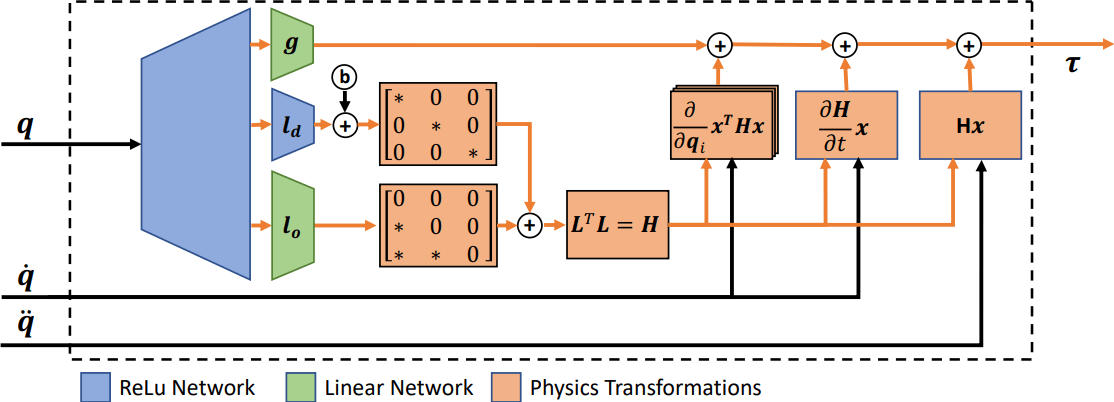
\includegraphics[width=0.8\textwidth]{slike/delan.png}
    \caption[DeLaN network architecture]{DeLaN network architecture \cite{Lutter2019}}
    \label{fig:DeLaN}
\end{figure}

A similar but more general method for learning arbitrary Lagrangians called Lagrangian Neural Networks (LNN) was presented in \cite{Cranmer2020}. Along with it, a good overview of neural network-based models for physical dynamics is given in the paper. It is shown that the complex model obtained by this approach successfully complies with the law of energy conservation. Furthermore, the obtained results show that the use of LNN almost strictly conserved the energy, unlike the baseline. The results were also compared to those obtained in \cite{Greydanus2019}, an approach inspired by Hamiltonian mechanics and showing similar performance, except that LNN can learn from arbitrary coordinates, while the method proposed in \cite{Greydanus2019} can only learn using canonical coordinates.

In \cite{Ledezma2017}, an approach called FOPnet was presented, which differs from classical neural networks for which the architecture is usually identified by trial and error. However, in the proposed approach, the network topology is determined from the physical characteristics of the dynamic system being modelled. Thus, this approach makes the topology (architecture) not subjective but dictated by the physics of the dynamic system. It was demonstrated how FOPnet for a robotic manipulator emerged from the Newton-Euler formulation for representing robot inverse dynamics. It showed that networks that compute dynamics and kinematics have weights that correspond to inertial and DH parameters of the robot.

The inverse dynamics of a robot is vital since models that are \emph{learned} can be used in place of analytical models that are usually required by the force estimation approaches based on observers, as emphasised previously in this section. 

An approach to learning the inverse dynamics of a robotic manipulator using Long-Short Term Memory (LSTM) networks at time $O(n)$ is presented in \cite{Rueckert2017}. This approach required an extensive data set of 100,000 samples, and using the proposed LSTM network, the prediction error decreases exponentially with the number of data samples used, and even for relatively small datasets, it shows better results than other modern approaches based on Gaussian processes. 

In \cite{Gupta2019} a novel framework for learning accurate dynamics of mechanical systems is proposed. The approach uses a ``grey-box'' model of a system in which the previous knowledge is incorporated where it is available, and otherwise, the estimators (i.e., neural networks) are trained. The ``grey-box'' model was used to address the variance vs bias issue, since the white-box model (i.e., parametrised, analytical model) introduces high bias and the black-box model (i.e., neural network) introduces high variance, as is shown in Figure \ref{fig:StructuredLearning}. The approach was applied on a simulated double pendulum but should be easily extendable to the field of robotics. However, the limitation of the method is that it is more computationally expensive than pure black- or white-box models.

\begin{figure}
    \centering
    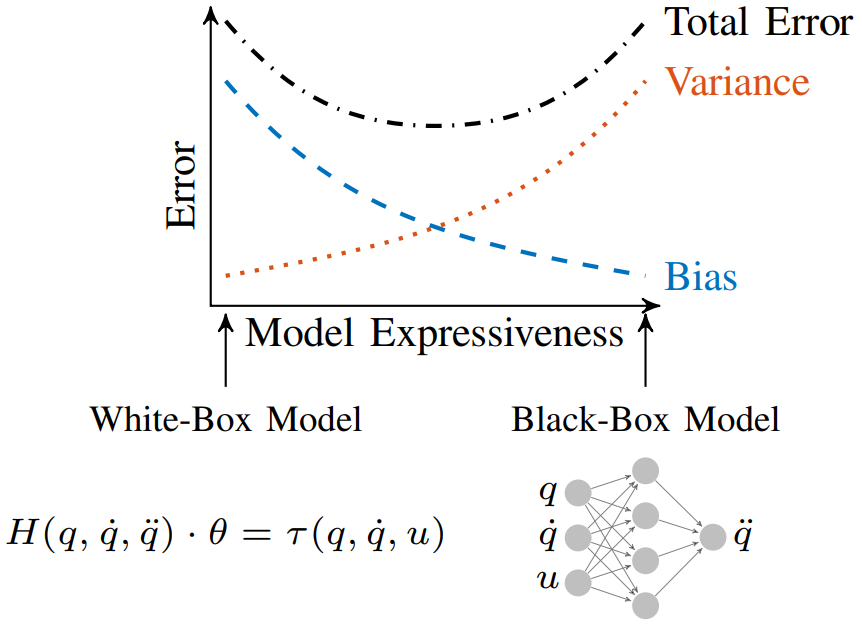
\includegraphics[width=0.5\textwidth]{slike/gupta2019.png}
    \caption[The bias-variance tradeoff]{The bias-variance tradeoff \cite{Gupta2019}}
    \label{fig:StructuredLearning}
\end{figure}

\newpage